\section{Experiments}\label{sec:experiments}
We evaluate intermediate feedback for composition, retention during sequential learning, and complete-task adaptation. The LIBERO-Spatial comparisons examine the feedback principle used in Section~\ref{sec:composition}; CDPR simulation evaluates retention and execution after adapting the action interface. The ongoing WX200 evaluation extends the approach to another embodiment.

\subsection{Intermediate Feedback for Full-Task Composition}\label{sec:libero_results}
Using the feedback variants in Section~\ref{sec:composition}, OpenVLA-OFT runs on the ten LIBERO-Spatial tasks share a 61.0\% initialization and use 300 validation rollouts per endpoint. The primary dense-and-phase and terminal-only conditions share the reported terminal verifier coefficient and 160-update budget. A low-success diagnostic starts at 2.0\%, measured over 1,000 rollouts, and compares dense feedback with terminal-only feedback over 20 updates using the same terminal-outcome group filter.

On the suite, dense-and-phase feedback reaches 65.3\% versus 61.7\% for terminal-only feedback. With terminal coefficient 1 and 110 updates, phase-only shaping reaches 62.3\%, while dense-and-phase shaping reaches 61.0\% (Table~\ref{tab:libero}). Their phase weights differ, so this is a comparison of reward configurations rather than an isolated test of reward density. The results show that intermediate events can support full-task learning, without establishing a universally best reward configuration.

On the low-success diagnostic, dense feedback reaches 18.0\% versus 11.0\% for terminal-only feedback from the same 2.0\% start. This comparison supports the use of dense feedback during initial acquisition. It does not select the final composition reward because no phase-only condition is reported for this task.

We select binary milestone feedback for composition on the design grounds in Section~\ref{sec:composition}: it retains intermediate credit while avoiding a separate continuous progress function for every phase of a new long-horizon instruction. Dense feedback remains part of initial skill acquisition. The low-success diagnostic and the full-suite phase comparison address these different roles within the pipeline.
\begin{table}[t]
\caption{LIBERO reward comparison. $\lambda$ is the terminal verifier coefficient; success and $\Delta$ are percentages and percentage-point gains. The low-success diagnostic tests initial learning, without a phase-only condition.}
\label{tab:libero}\centering\small
\begin{tabular}{@{}lrrr@{}}\toprule
Configuration & Updates & Success & $\Delta$\\\midrule
\multicolumn{4}{@{}l}{LIBERO-Spatial: initial 61.0\%}\\
Terminal only, $\lambda=5$ & 160 & 61.7 & +0.7\\
Dense + phase, $\lambda=5$ & 160 & 65.3 & +4.3\\
Filtered dense + phase, $\lambda=5$ & 50 & 64.7 & +3.7\\
Dense + phase, $\lambda=1$ & 110 & 61.0 & +0.0\\
Phase-only shaping, $\lambda=1$ & 110 & 62.3 & +1.3\\
\midrule
\multicolumn{4}{@{}l}{Low-success diagnostic: initial 2.0\% (1,000 rollouts)}\\
Terminal only & 20 & 11.0 & +9.0\\
Dense mixture & 20 & 18.0 & +16.0\\
\bottomrule
\end{tabular}
\end{table}



% Queue the retention float early enough to stay near its results.
\begin{figure*}[!t]
\centering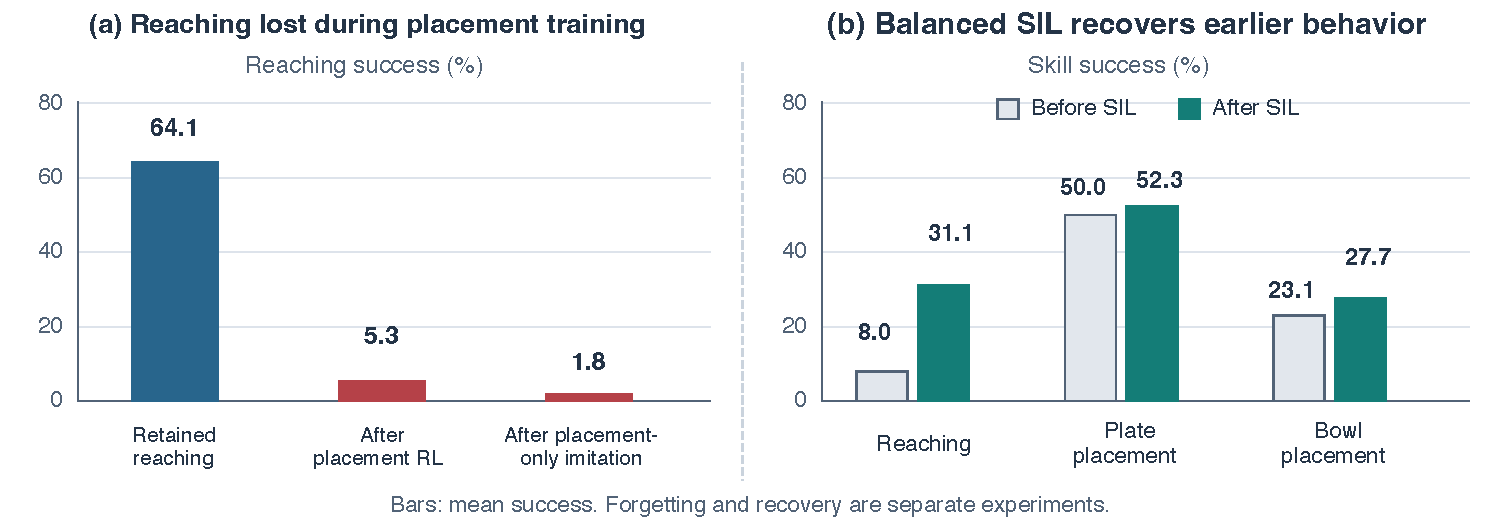
\includegraphics[width=\textwidth]{figures/skill_retention.pdf}
\caption{Skill success before and after balanced self-imitation. Bars show means across three evaluation rounds for reaching and two rounds for each placement skill, per condition. Reaching partially recovers while both placement means increase.}
\label{fig:retention}
\end{figure*}

\subsection{SmolVLA: Complete-Task Adaptation}\label{sec:cdpr_results}
The CDPR simulation uses MuJoCo Warp/MJ-Lab, four object categories (apple, orange, potato, and tomato), and plate or bowl destinations. The action interface controls Cartesian translation, yaw, and the gripper. Strict success requires grasp, held lift, intentional release, and correct placement, without carry slip or wrong-placement events.

The development validation comprises 1,024 full-task episodes: 512 plate and 512 bowl attempts. Each attempt starts with an empty gripper and uses one full-task instruction, without teacher assistance. All attempts, including numerical failures, remain in the denominator.
The adapted controller completes 723 of 1,024 development validation attempts (70.61\% strict success; Table~\ref{tab:cdpr}). Physical grasp occurs in 92.48\% of attempts and held lift in 88.28\%. Completion rates are 393/512 (76.76\%) for plates and 330/512 (64.45\%) for bowls. Carry slips (16.70\%) and wrong placements (14.16\%) remain the main failure modes.
\begin{table}[t]
\caption{CDPR complete task development evaluation.}
\label{tab:cdpr}\centering\small
\begin{tabular}{@{}lr@{}}\toprule
Outcome & Attempts (\%)\\\midrule
Physical grasp & 92.48\\
Held lift & 88.28\\
Strict completion (723/1,024) & 70.61\\
Carry slip & 16.70\\
Wrong placement & 14.16\\\bottomrule
\end{tabular}
\end{table}


\subsection{Skill Recovery with Balanced Self-Imitation}
Balanced self-imitation raises reaching success from 8.0\% to 31.1\% (Fig.~\ref{fig:retention}). Plate placement changes from 50.0\% to 52.3\%, and bowl placement from 23.05\% to 27.65\%. The bank combines earlier reaching successes with current placement successes. Each skill is evaluated under its own fixed reset protocol; placement skill tests can begin with a held object.


Recovery is partial, with placement performance retained while reaching improves. These skill-level results do not isolate the contribution of self-imitation to final full-task success.


\subsection{Additional Embodiment: WX200}\label{sec:wx200}
An ongoing experiment applies the pipeline to the five-DoF WX200 serial manipulator. This setting changes the robot mechanism while retaining the skill-learning and composition schedule. Figure~\ref{fig:wx200} reserves the setup and rollout illustrations. Quantitative success rates will be added after the evaluation is complete.

\begin{figure*}[!t]
\centering
\IfFileExists{figures/wx200/panel.pdf}{\includegraphics[width=\textwidth]{figures/wx200/panel.pdf}}{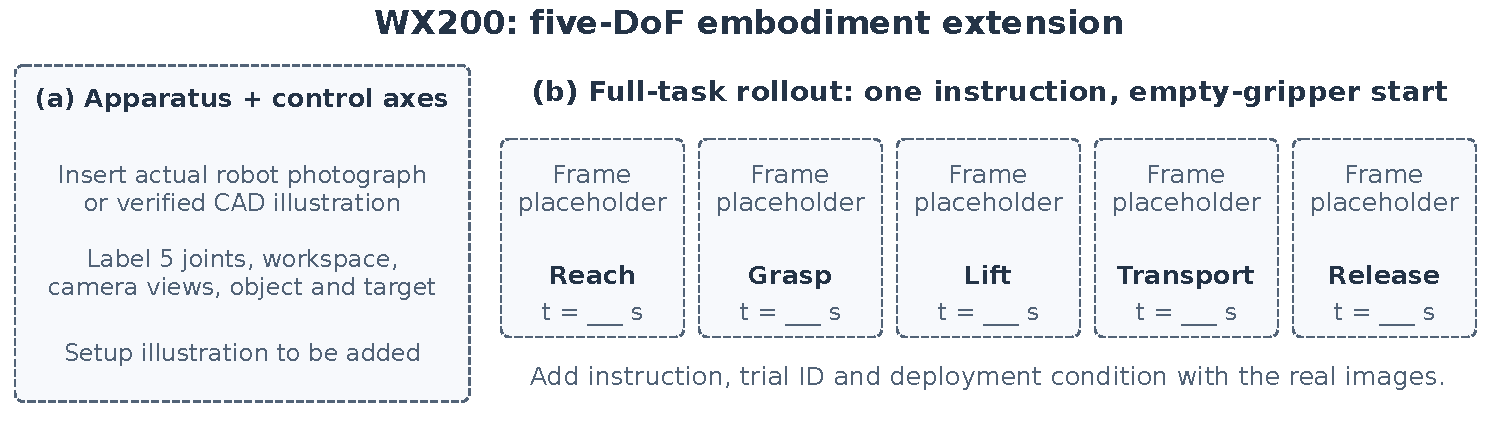
\includegraphics[width=\textwidth]{figures/wx200_slots.pdf}}
\caption{WX200 evaluation layout. (a) Apparatus, workspace, cameras, and control axes. (b) Reach, grasp, lift, transport, and release under one instruction. The current panels reserve space for setup images and timestamped rollout frames from the ongoing experiment.}
\label{fig:wx200}
\end{figure*}

\subsection{Scope of the Evidence}
The experiments evaluate connected parts of the adaptation procedure under their respective protocols. The LIBERO comparisons examine intermediate feedback for composition; the CDPR results measure skill recovery and complete-task execution after action-interface adaptation. The complete-task result comes from one SmolVLA training lineage and a development validation panel used during training. Retention measurements cover a small number of rounds, and the experiments do not isolate every stage of the pipeline. Earlier assisted training is part of the inherited CDPR policy; the reported full-task evaluation uses no assistance.

